% Task 2: jump to the middle of an encrypted film. Values from Task2/jump.py and Task2/film.bin.
% CHECKED (python3, Task2/chacha.py, key 5eed..., nonce 00..02):
%   film.bin has 64 000 bytes = 1000 blocks of 64 bytes; block n was encrypted with counter n.
%   the first bytes of blocks 0, 1, 2, 699, 700, 701, 999:
%     4D A0, D7 96, 25 1C, 23 6D, 98 72, 1C 7E, 55 BC
%   block 700 = bytes 44 800 to 44 863; with counter 700 it decrypts to "Frame 0700: ..." (the result: not shown)
\documentclass[12pt,tikz,border=6pt]{standalone}
% Shared preamble of the task figures of Lecture 2 (a copy of Lecture01-RC4/task-figures/common.tex).
% The colours and styles are copied from the preamble of ../main.tex (keep them in sync).
% The ChaCha20 roles take the colours of the ChaCha20 simulator (CryptographySimulators/chacha20),
% so that the README figures and the simulator look the same:
%   key: amber, nonce: blue, counter: green, constants: grey, ciphertext: violet, a change: orange.
\usepackage{lmodern}
\usepackage[T1]{fontenc}
\renewcommand{\familydefault}{\sfdefault}
\usepackage{amsmath,amssymb}
\usepackage{xcolor}
\usepackage{fontawesome5}
\usetikzlibrary{arrows.meta, calc, positioning, fit, decorations.pathreplacing, decorations.pathmorphing, backgrounds}

% ---------- template ----------
\definecolor{DeepBlue}{HTML}{283593}
\definecolor{AccentOrange}{HTML}{EB5A14}
\definecolor{LightGray}{HTML}{F5F6FA}
% ---------- actors and categories (S1 to S6) ----------
\definecolor{sIndigo}{HTML}{5C6BC0}   % the sender
\definecolor{sPink}{HTML}{EC407A}     % the attacker
\definecolor{sViolet}{HTML}{7E57C2}   % plaintext
\definecolor{sAmber}{HTML}{FFB300}    % key and keystream
\definecolor{sTeal}{HTML}{26A69A}     % the receiver
\definecolor{sBrown}{HTML}{8D6E63}    % ciphertext
\definecolor{sPinkText}{HTML}{C2185B}
\definecolor{sAmberText}{HTML}{A06A00}
\definecolor{sTealText}{HTML}{00796B}
% ---------- actions and results ----------
\definecolor{aExec}{HTML}{43A047}
\definecolor{aRead}{HTML}{1E88E5}
\definecolor{aWrite}{HTML}{E53935}
% ---------- neutral ----------
\definecolor{nInk}{HTML}{37474F}
\definecolor{nLine}{HTML}{90A4AE}
\definecolor{nLight}{HTML}{CFD8DC}
\definecolor{nFill}{HTML}{ECEFF1}
\definecolor{nIdle}{HTML}{E0E0E0}

% ---------- TikZ styles (as in main.tex; byte cells a little larger for the web) ----------
\tikzset{
  hw/.style={draw=nLine, thick, fill=nFill, text=nInk, rounded corners=3pt, align=center, inner sep=4pt},
  hwmain/.style={draw=nInk, thick, fill=nInk, text=white, rounded corners=3pt, align=center, inner sep=4pt},
  cell/.style={draw=nLine, thick, fill=white, text=nInk, font=\ttfamily\small},
  cellfree/.style={cell, dashed, draw=nLight},
  container/.style={draw=nLine, thick, dashed, rounded corners=5pt},
  actor/.style={fill=#1, draw=#1, text=white, rounded corners=3pt, align=center, font=\small\bfseries, inner sep=5pt},
  actorlight/.style={fill=#1!15, draw=#1, thick, text=nInk, rounded corners=3pt, align=center, inner sep=5pt},
  data/.style={-{Stealth}, very thick, nInk},
  flow/.style={-{Stealth}, very thick, DeepBlue},
  annot/.style={draw=AccentOrange, line width=1.6pt, rounded corners=3pt},
  byte/.style={draw=nLine, thick, fill=white, text=nInk, font=\ttfamily\small,
    minimum width=0.8cm, minimum height=0.62cm, inner sep=1pt, rounded corners=1.5pt},
  ptb/.style={byte, fill=white, draw=nInk},   % plaintext: neutral here, violet is the ciphertext
  ksb/.style={byte, fill=sAmber!25, draw=sAmber},
  rowlabel/.style={font=\small\bfseries, text=nInk, anchor=east},
  note/.style={font=\small, text=nInk},
  bigxor/.style={circle, draw=nInk, very thick, fill=white, inner sep=0pt, minimum size=0.8cm, font=\Large},
  radio/.style={-{Stealth}, very thick, nInk, decorate,
    decoration={snake, amplitude=1.2pt, segment length=7pt, post length=4pt}},
  % a white card behind the whole figure, so that it stays readable in a dark theme
  card/.style={show background rectangle, background rectangle/.style={fill=white, draw=none}, inner frame sep=8pt},
}
% a row of bytes: \byterow{x of the first cell}{y}{style}{list of values}{step between cells}
\newcommand{\byterow}[5]{%
  \expandafter\def\expandafter\brlist\expandafter{#4}%
  \foreach \v [count=\k from 0] in \brlist {
    \node[#3] at ({#1+#5*\k},#2) {\v};
  }}
% the generator / cipher box: dark, with cogs. \cogbox{name}{position}{label}{width}
\newcommand{\cogbox}[4]{%
  \node[hwmain, minimum width=#4, minimum height=1.3cm] (#1) at (#2) {};
  \node[text=white, font=\Large] at ([yshift=0.22cm]#1.center) {\faCogs};
  \node[text=white, font=\small\bfseries] at ([yshift=-0.32cm]#1.center) {#3};}
\newcommand{\ok}{\textcolor{aExec}{\faCheck}}
\newcommand{\nok}{\textcolor{aWrite}{\faTimes}}
\newcommand{\badge}[1]{\tikz[baseline=(b.base)]\node[circle,fill=AccentOrange,text=white,
  inner sep=1.5pt,font=\bfseries\footnotesize] (b) {#1};}

% ---------- ChaCha20 roles (the colours of the ChaCha20 simulator) ----------
\definecolor{rKey}{HTML}{E2A60E}    \definecolor{rKeyBg}{HTML}{FDF3DC}
\definecolor{rNonce}{HTML}{2F6FDB}  \definecolor{rNonceBg}{HTML}{E5EDFB}
\definecolor{rCtr}{HTML}{2FA84F}    \definecolor{rCtrBg}{HTML}{E3F4E8}
\definecolor{rConst}{HTML}{BCC4CC}  \definecolor{rConstBg}{HTML}{EEF1F4}
\definecolor{rCt}{HTML}{8A5CD8}     \definecolor{rCtBg}{HTML}{F1EAFD}
\definecolor{rKeyText}{HTML}{9A6B00}
\definecolor{rNonceText}{HTML}{1F55B5}
\definecolor{rCtrText}{HTML}{1E7E4F}
\definecolor{rCtText}{HTML}{6A3FB8}
\definecolor{rChg}{HTML}{D9621C}
\tikzset{
  keyb/.style={byte, fill=rKeyBg, draw=rKey},
  nonceb/.style={byte, fill=rNonceBg, draw=rNonce},
  ctrb/.style={byte, fill=rCtrBg, draw=rCtr},
  ctb/.style={byte, fill=rCtBg, draw=rCt},
  chg/.style={byte, fill=AccentOrange!18, draw=AccentOrange, line width=1.4pt, font=\ttfamily\small\bfseries},
  unk/.style={byte, fill=white, dashed, text=nInk},
  inbox/.style={draw=#1, thick, fill=#1!12, text=nInk, rounded corners=3pt, align=center, inner sep=5pt},
}

\begin{document}
\pagecolor{white}
\begin{tikzpicture}[>=Stealth]
  \def\w{1.55}
  % one frame of the film strip: \frame{x}{block number}{first bytes}{byte offset}{style extra}
  \newcommand{\filmblock}[5]{%
    \fill[nInk] ({#1-\w/2},-0.95) rectangle ({#1+\w/2},0.95);
    \foreach \h in {-0.5,-0.2,0.1,0.4} {
      \fill[white] ({#1+\h*\w/1.1-0.06},0.72) rectangle ({#1+\h*\w/1.1+0.06},0.84);
      \fill[white] ({#1+\h*\w/1.1-0.06},-0.84) rectangle ({#1+\h*\w/1.1+0.06},-0.72);}
    \node[draw=rCt, thick, fill=rCtBg, minimum width={\w cm-0.22cm}, minimum height=1.2cm, rounded corners=1pt, #5] at (#1,0) {};
    \node[font=\scriptsize\bfseries, text=nInk] at (#1,0.25) {block #2};
    \node[font=\ttfamily\scriptsize, text=rCtText] at (#1,-0.2) {#3};
    \node[ctrb, minimum width=1.25cm, font=\ttfamily\scriptsize] at (#1,-1.45) {ctr #2};
    \node[font=\scriptsize, text=gray] at (#1,1.2) {byte #4};}
  \newcommand{\gap}[1]{%
    \fill[nInk] ({#1-0.45},-0.95) rectangle ({#1+0.45},0.95);
    \node[text=white, font=\large] at (#1,0) {\ldots};}

  % title
  \node[font=\normalsize\bfseries, text=nInk, anchor=west] at (-1.0,2.75)
    {\faFilm\ \texttt{film.bin}: 1000 blocks of 64 bytes = 64\,000 bytes of ciphertext};

  \filmblock{0.0}{0}{4D A0}{0}{}
  \filmblock{1.6}{1}{D7 96}{64}{}
  \filmblock{3.2}{2}{25 1C}{128}{}
  \gap{4.5}
  \filmblock{5.8}{699}{23 6D}{44\,736}{}
  \filmblock{7.4}{700}{98 72}{44\,800}{draw=AccentOrange, line width=2pt, fill=AccentOrange!15}
  \filmblock{9.0}{701}{1C 7E}{44\,864}{}
  \gap{10.3}
  \filmblock{11.6}{999}{55 BC}{63\,936}{}
  \node[note, anchor=west, text=rCtrText, align=left] at (12.55,-1.45) {block $n$ was encrypted\\ with counter $n$};

  % the slow way: all blocks from the start
  \draw[nLine, line width=5pt] (-0.75,1.7) -- (8.0,1.7);
  \draw[-{Stealth}, nLine, line width=2pt] (7.9,1.7) -- (8.3,1.7);
  \node[note, anchor=west] at (8.45,1.7)
    {\textcolor{nLine}{\faHourglassHalf}\ \textbf{slow:} all 701 blocks, counter 0 to 700};

  % the fast way: jump to block 700
  \draw[-{Stealth}, AccentOrange, line width=2pt] (7.4,-1.8) -- (7.4,-3.05);
  \node[font=\small\bfseries, text=AccentOrange, anchor=west] at (7.55,-2.4) {\faBolt\ fast: jump straight to block 700};
  \node[actorlight=rKey, font=\small, minimum height=0.65cm] (k) at (3.7,-3.45) {\faKey\ key};
  \node[inbox=rNonce, font=\small, minimum height=0.65cm] (n) at (5.3,-3.45) {nonce};
  \node[ctrb, minimum width=2.1cm, minimum height=0.65cm, font=\ttfamily\small\bfseries, draw=AccentOrange, line width=1.4pt] (c) at (7.4,-3.45) {counter 700};
  \node[hwmain, minimum width=3.2cm, minimum height=1.2cm] (cc) at (10.9,-3.45) {};
  \node[text=white, font=\Large] at (9.85,-3.45) {\faCogs};
  \node[text=white, font=\normalsize\bfseries] at (11.25,-3.45) {ChaCha20};
  \draw[data] (c) -- (cc);
  \draw[decorate, decoration={brace, mirror, amplitude=5pt}, nInk] (2.95,-3.9) -- (8.45,-3.9)
    node[midway, below=6pt, font=\scriptsize, text=nInk] {the same key and nonce as the whole film};
  \node[font=\scriptsize, text=nInk, anchor=north] at (10.9,-4.1) {only 64 bytes in};
  \draw[data] (12.5,-3.45) -- (13.3,-3.45);
  \node[font=\ttfamily\small, text=nInk, anchor=west] at (13.35,-3.45) {Frame 0700: ? ? ?};
\end{tikzpicture}
\end{document}
